%Review of timbral control research.
%	Timbre Definition
%	Timbre Spaces (MDS and shit)
%	Audio Features
%	Perceptual Control of Synthesis

\chapter{Timbre}
\label{chap:Timbre}
	There are three properties which describe how a sound is perceived, these being loudness, pitch and timbre. Loudness
	describes the perceived intensity of a sound and pitch its perceived frequency. Timbre then describes any other
	properties of a sound, besides loudness and pitch, which allow it to be distinguished from other sounds
	\citep{mathews1999introduction}. Loudness and pitch are both one dimensional properties allowing sounds to be
	ordered from quiet to loud or low to high pitch. Timbre is a more complex property consisting of multiple dimensions
	\citep{rossing2002the}. There is a large body of research concerning the analysis of timbre, identifying these
	dimensions and their relationships with the acoustic features of a sound.

	Simple descriptions of a sounds timbre involve instrument identification. A sound could be described as `cello-like'
	or `flute-like'. More broadly the class of instrument, string or woodwind, could be used to describe the timbre of a
	sound. While these terms are useful for discussing the instrumentation of pieces they can not be applied generally
	to a wide range of timbres. It is not very useful to describe the timbre of a xylophone as being `not flute-like'.

	More general timbral descriptors directly describe the sound itself rather than the source which produced it. These
	include terms such as bright, rough and sharp. This allows the timbre of different sounds to be compared according
	to these terms \citep{howard2009acoustics}. Sounds can also be ordered in respect to these criteria much like with
	loudness and pitch. For example one could order a set of sounds by how bright they sound.

	Early research into timbre was performed by \citet{helmholtz1875on}. More recent work involves research from various
	fields. Low level features of audio segments can be found using signal analysis techniques. More complicated
	information about the perception of a signal can be discovered through modelling the behaviour of the human hearing
	system. Lastly experiments can be undertaken in which participants listen to audio samples and provide responses
	regarding the timbre of the samples. These responses are then analysed to uncover any correlations between the
	participants responses and lower level features of the audio samples.

	This chapter will review the existing body of timbral research. Section \ref{sec:Timbre-LowLevelFeatures} discusses
	metric which are used to describe the low level features of audio signals. Section
	\ref{sec:Timbre-PsychoacousticPrinciples} covers various models which describe the perception of various auditory
	phenomena. \note{Put in what the rest of the sections are about}.

\section{Low Level Audio Features}
\label{sec:Timbre-LowLevelFeatures}
	A widely cited definition of timbre \citep{ASA1960american} suggests that timbre in influenced by various low level
	features of an audio signal. The spectral content, waveform and temporal characteristics all effect the perceived
	timbre of a sound. Signal analysis techniques can be used to extract information about these elements of a signal.
	A large list of such features feature extraction techniques is given by \citep{peeters2004a}. These features can be
	separated into three categories. Features which describe the properties of a signals waveform and how it evolves
	with time (temporal features), features which describe the frequency content of a signal (spectral features) and
	features which describe how the frequency content of a signal evolves with time (spectro-temporal features). 

	\subsection{Temporal Features}
	\label{sec:Timbre-LowLevelFeatures-Temporal}
		Simple temporal features involve taking statistical measurements, such as mean and variance, of the audio
		samples in a signal. These measures give basic information about the level and variation in a signal but in
		many cases they do not represent a signals properties very well. For example, the mean value of a sinusoidal
		signal over a whole number of cycles is zero. 

		A common technique to extract more meaningful information about a signals level is to use an envelope
		detector. An envelope detector extracts the amplitude envelope of a signal. The amplitude envelope provides
		information about the level of a signal over time. An example amplitude envelope is shown in Figure
		\ref{fig:AmplitudeEnvelope}.

		\begin{figure}[h!]
			\centering
			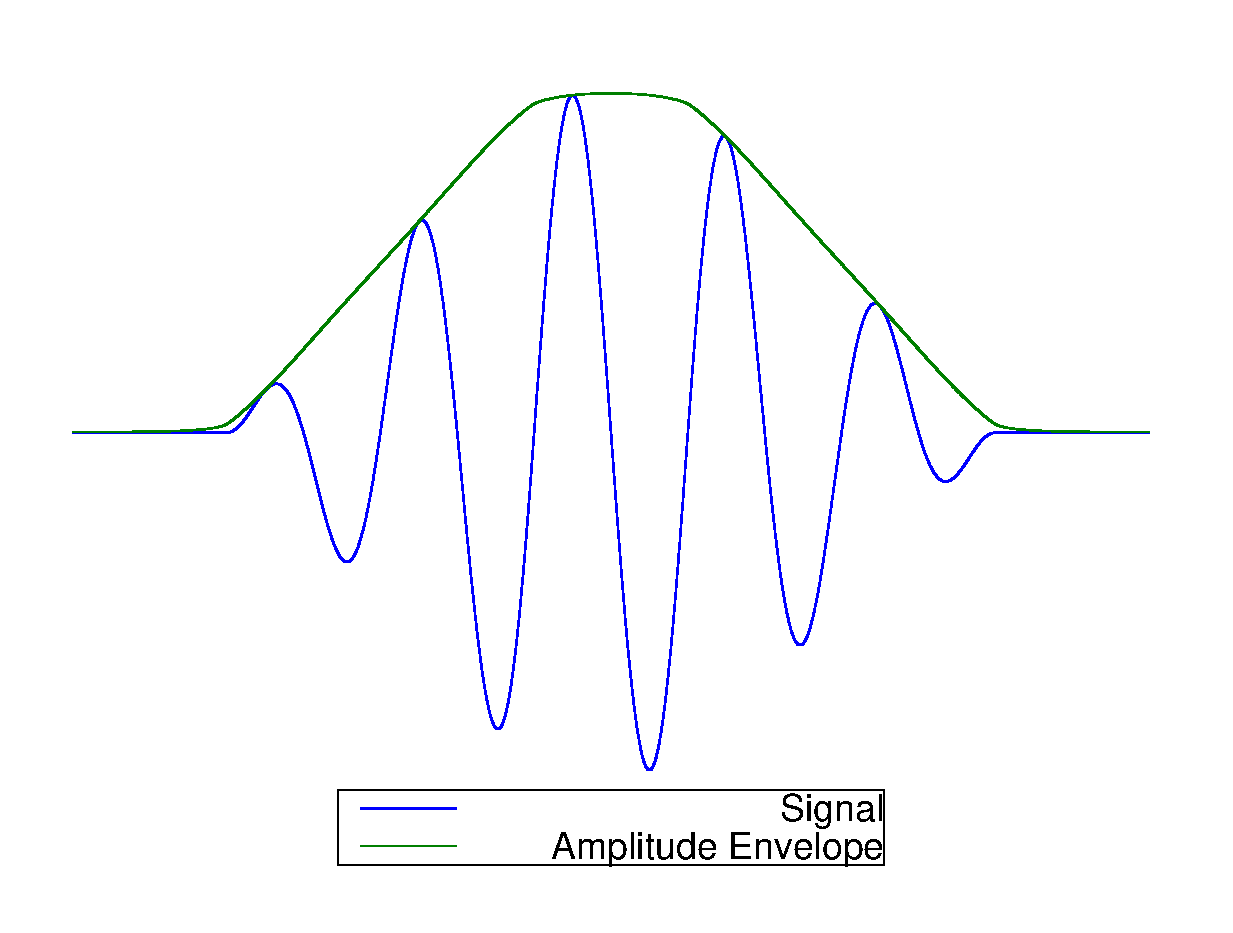
\includegraphics[width=0.6\textwidth]{chapter2/Images/AmplitudeEnvelope.eps}
			\caption{The Amplitude Envelope of a Signal.}
			\label{fig:AmplitudeEnvelope}
		\end{figure}

		Various envelope detection methods are reviewed by \citet{chang2007a}. \citet{howard2009acoustics} separates
		the envelope of a sound into three sections. The steady state section is the middle portion in which the
		timbre of the sound only varies slightly. The onset and offset sections describe the way the sound rises
		from silence to the steady state and returns to silence after. Further refinement of the description of
		amplitude envelopes leads to the ADSR (Attack, Decay, Sustain, Release) model \citep{descrivan2012music}. An
		example ADSR envelope is shown in Figure \ref{fig:ADSR}.

		\begin{figure}[h!]
			\centering
			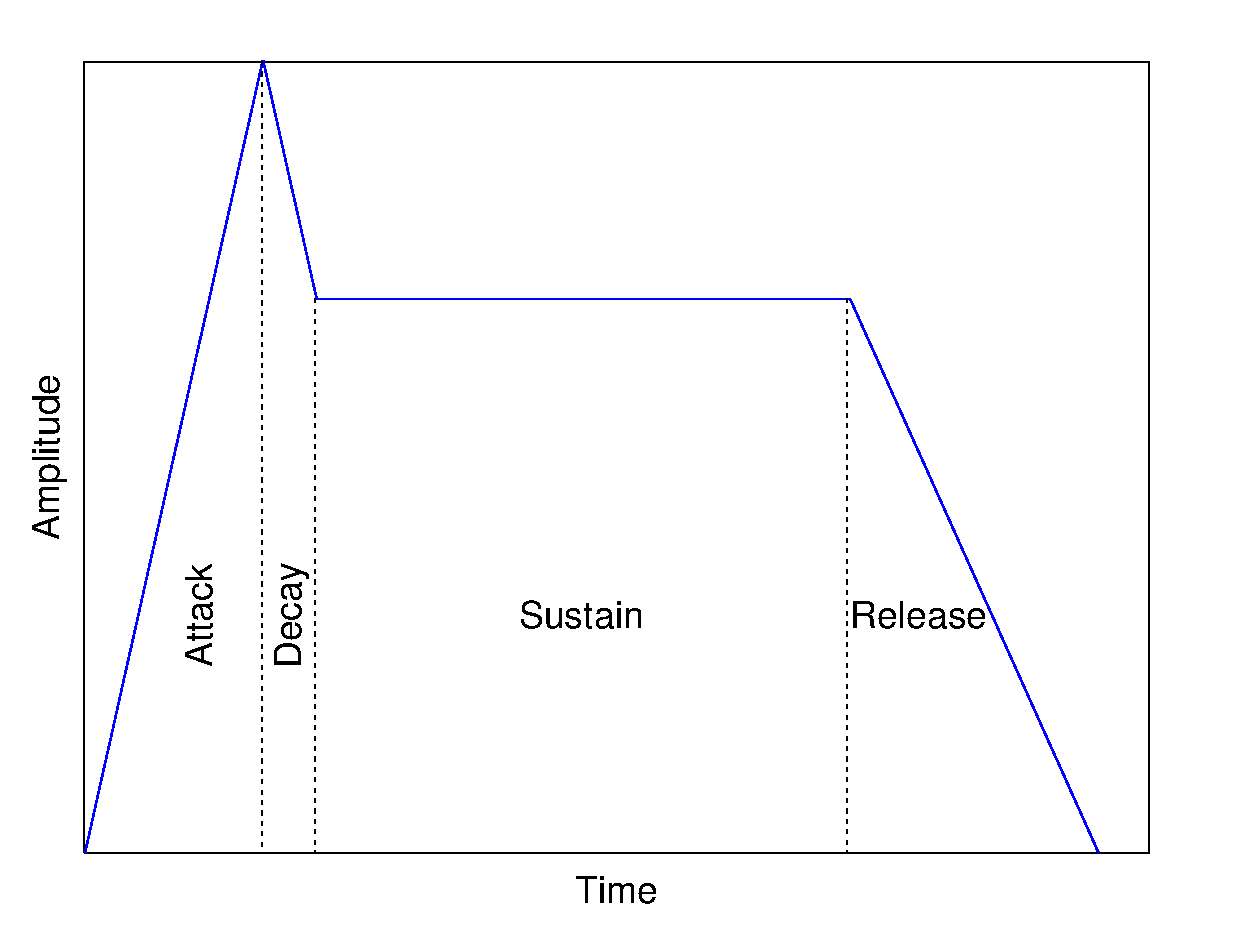
\includegraphics[width=0.6\textwidth]{chapter2/Images/ADSR.eps}
			\caption{An ADSR Envelope.}
			\label{fig:ADSR}
		\end{figure}

		Once the amplitude envelope of a signal has been extracted further statistics can be calculated from it such
		as log attack time and temporal centroid \citep{peeters2000instrument}.

	\subsection{Spectral Features}
	\label{sec:Timbre-LowLevelFeatures-Spectral}
		\note
		{
			\begin{itemize}
				\item Spectral statistics.
				\item Spectral shape.
				\item MFCCs.
			\end{itemize}

			MFCCs originally developed for speech recognition \citep{davis1980comparison} but used for other
			timbral tasks more recently \citep{depoli1997sonological}.
		}

	\subsection{Spectro-Temporal Features}
	\label{sec:Timbre-LowLevelFeatures-Spectrotemporal}
		\note
		{
			Delta MFCC and spectral flux and such and the like.
		}

	\note
	{
		Stuff like this also \citep{freed1990auditory, lakatos2000a}.
	}
	
\section{Psychoacoustic Principles}
\label{sec:Timbre-PsychoacousticPrinciples}
	Psychoacoustics is a field which deals with the perception of sound. The existing literature concerns the study of
	the human hearing system and how it responds to certain aspects of audio stimuli. Several different areas of audio
	perception have been researched. Methods have been devised to model the human perception of loudness
	\citep{moore1997a} and pitch \citep{gerhard2003pitch}. Other research considers the human hearing systems ability to
	locate sound sources \citep{blauert1997spatial}. This section will summarise the psychoacoustic principles which are
	useful for investigating the perception of timbre. 

	\note
	{
		Critical bands and masking.

		Resolving harmonics in the cochlea. Low order harmonics are generally resolved individually so their
		individual levels will have a strong effect on perceived timbre. Higher order harmonics are resolved in
		groups so less manipulation is needed \citep{howard2009acoustics}.
	}

\section{Timbral Features}
\label{sec:Timbre-TimbralFeatures}
	\note
	{
		Psychoacoustic principles have been used to develop timbral metrics (sharpness, roughness).
	}

\section{Parameterisation of Timbre}
\label{sec:Timbre-Parameterisation}
	\note{Analysis of timbre spaces and discussion on salience of some features as given in the literature.}

	\subsection{Dissimilarity Tests}
	\label{sec:Timbre-Dissimilarity}
		\note
		{
			A more traditional approach, \citet{grey1977multidimensional} and all the copycat lot 
			\citep{burgoyne2008a, caclin2005acoustic}.
		}

	\subsection{VAME}
	\label{sec:Timbre-VAME}
		\note{\citet{kendall1993verbal1, kendall1993verbal2} trying to upset the status quo.}

	\subsection{Parameter Space}
	\label{sec:Timbre-ParameterSpaces}
	\note{Research like Social EQ and stuff \citep{cartwright2013socialeq, seetharaman2014crowdsourcing}.}

\section{Controlling Timbre}
\label{sec:Timbre-Control}
	\note{Lots of them synthesis dudes have tried to control the beast. \citet{zacharakis2011an} did some stuff.}
	
	\note
	{
		Some dudes do morphing (analysis resynthesis from what I remember) like good old 
		\citet{williams2007perceptually, williams2009perceptually, williams2010perceptually}
	}
